\chapter{Cupria, a novel cell-free system for industrial biotechnology}

\section{\textbf{Abstract }}

Cell-free systems (CFS) are an emerging technology where cell extracts are used instead of living genetically-modified cells, thus, not presenting a "living prospect" applicable to current legal regulations.  Here we show a versatile cell-free system based on the master survivalist bacteria \textit{Cupriavidus  metallidurans} CH34, able of not only sensing environmental variables, such as heavy metals, but also synthesize proteins, produce bioplastics and degrade toxic aromatic compounds. This novel cell-free  chassis  could  become  a  standard  for  mass production considering the versatility and robustness showed once compared with standard \textit{E. coli} cell-free systems. 

lala\footnote{testing a footnote}.

\section{\textbf{Introduction }}

While cell based systems have to be a self-replicating chassis as its greater advantage, cell-free expression systems are a powerful tool in applications where cell based expression systems are too variable, slow, difficult to store or prohibitive due to legislation on the release of genetically modified organisms. 

Since interaction with the surrounding environment is direct

As their very nature is to be a defined, precisely controlled system, their lack of a self-replicating functionality, allows them to function in a limited supply of intracellular supplies such as ATP sources, amino acids and nucleotides. In consequence in vitro protein synthesis is limited by two dimensions: the overall maximum protein amount that can be synthesized with the supplied components, and the time during which the cell free expression system stays active before background processes and chemical deterioration have used up supplies or inactivated the system (\cite{carlson2012cell,bernhard2013cell,kwon2015high}.
\section{\textbf{Methodology }}

\subsection*{Strains and Cell free extract preparation}

\textit{E. coli} MG1655 and \textit{C. metallidurans} CH34 strains were grown on Luria Broth (LB) at 37$^{\circ}$C and 30$^{\circ}$C respectively, both under constant shaking at 180 RPM. Cultures were induced with the respective heavy metal at middle exponential phase and cells collected by centrifugation at 10.000 RPM, 4 C for 5 min. Resuspension was performed using Tris-HCl (40 mM) pH 7.5, followed by a nonionic lysis step using Triton X-100 (0.8\%), Tris-HCl (40 mM) pH 7.5 and lysosime 50 mg/mL. Lysed was centrifuged at 10.000 RPM, 4$^{\circ}$C for 10 min and supernatant was saved at -80$^{\circ}$C or immediately used.

\subsection*{DNA constructs generation}
Promoters from clusters \textit{copAB}, \textit{arsBCD} from E. coli MG1655 and \textit{merTPAD}, \textit{pbrAB} from C. metallidurans CH34 were added by PCR at the 5’ of the pTUB[F30::iSpinach] aptamers using the Q5 High-Fidelity DNA Polymerase (NEB). Transcriptional regulators MerR, PbrR, ArsR and CueR were provided in to the working reaction directly from the cell extract.
pBP, pTUB (Moore et al., 2016), pSB1, pSB4 (iGEM collection), pGEM (Promega), pET28, pET31 (Paige et
al., 2011), ptZ57R/T (Autour et al., 2016), pMO (Kuehl et al., 2014), pSEVA (Silva-Rocha et al., 2013)
plasmids were used as backbones. All constructs generated were confirmed by Sanger sequencing(Edinburgh Genomics). Primer sequences are listed in Appendix 2. Plasmids were digested using
appropriate restriction enzymes (NEB) and excised from agarose 1.3 - 2\% gel, and recovered using a
Quiaquick gel extraction kit (Quiagen). Ligation steps were performed using T4 DNA ligase and 30 fmol of
plasmid per 90 fmol of insert (1:3). Ligations were used to transform chemically competent E. coli JM109
cells selected on the appropiate antibiotic, plasmid DNA was prepared
using a QIAprep Spin Miniprep Kit
(Qiagen) and constructs further confirmed by PCR and Sanger sequencing.
Constructs for expressing crRNA (Figure 10) and the F30 scaffold were synthesized (Sigma-Aldrich) and
cloned in to pBP (Figure 7). All RNA aptamers generated by Paige et al., (2011) and Autour (2017), except
Spinach, were cloned by Golden gate assembly in pTUB flanked by an F30 scaffold (Figure 8). Nullomers 2
(5’ GTCCGAGCGTA 3’) and 5 (5’ ATGTTGATGTTGT 3’) (see Table 6) were cloned flanking the
F30::iSPinach construct in the pGEMTeasy by TA cloning (Figure 11 and 12), using Platinum Taq
polymerase High Fidelity (ThermoFisher). Promoters from the copAB and arsBCD operons from E. coli
MG1655 and merTPAD, pbrAB operons from C. metallidurans CH34 were added by PCR on the 5’ end of
the F30::Broccoli (pET28C) and F30::iSpinach (pTUB) aptamers using Q5 High-Fidelity DNA Polymerase
(NEB). Plasmids were transformed into chemically competent E. coli as prepared by the standard TSS
method (Chung et al., 2014).

\subsection*{Expression and detection of Fluorescent RNA aptamers.}

Although there are standard protocols for in vitro transcription of fluorescent RNA aptamers, these include purification and concentration steps that complicate the entire procedure. A combination of both main steps was achieved at room temperature (25$^{\circ}$C) using our Optimized Transcription/Detection buffer (OTDB): Tris-HCl (40 mM) pH 7.5; MgCl2*6(H2O) (6 mM); DTT (1 mM); Spermidine (2 mM); NTPs (2 mM each); DFHBI (20 uM); NEB T7 RNA polymerase (1.5 U/uL); Template DNA (650 nM). 
Fluorescence was measured using a FluoStar Omega (BMG Labtech) plate reader, excitation 480 nm/ emission 520 nm filters (10 mm bandpass), using 20 flashes per well and an orbital averaging of 4 mm, with 5 seconds of orbital shaking prior each measurement. 

\subsection*{Heavy metal quantification by fluorescence detection}
Stock solutions (100 mM) of HgCl 2 (Sigma-Aldrich), CuSO 4 • 5H 2 O (Sigma-Aldrich), ZnSO 4 • 7H 2 O
(Sigma-Aldrich), CdSO 4 (Sigma-Aldrich), Na 2 HAsO 4 • 7H 2 O (Sigma-Aldrich), Pb(NO 3 ) 2 (VWR), NaAsO 2
(HoneyWell) were prepared and used according to their free metal ion concentration (Table 1).
Table 1: Metal stock solution with their free ion concentrations.
Metal solution Concentration ppm Free Ion Concentration ppm
HgCl 2 100 mM 27152 Hg +2 100 mM 20059
CuSO 4 •5H 2 O 100 mM 24969 Cu +2 100 mM 6355
Pb(NO 3 ) 2 100 mM 33120 Pb +2 100 mM 20720
ZnSO 4 •7H 2 O 100 mM 28756 Zn +2 100 mM 6538
CdSO 4 100 mM 20487 Cd +2 100 mM 11241
Na 2 HAsO 4 •7H 2 O 100 mM 31201 As +5 100 mM 7492
NaAsO2 100 mM 12991 As +3 100 mM 7492

\section{\textbf{Results}}

%\begin{figure}[htbp]
 % \centering
%  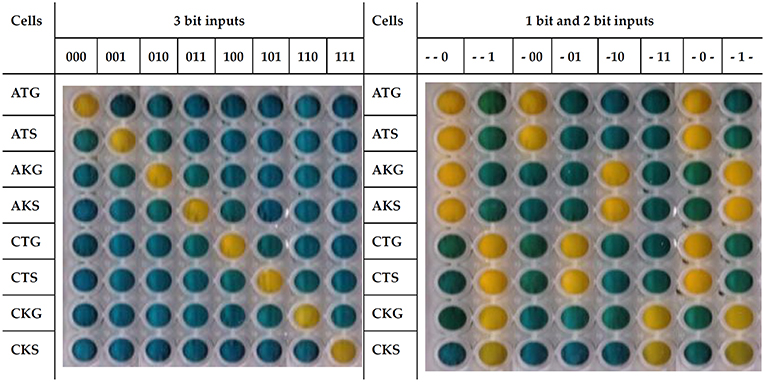
\includegraphics[width=0.7\textwidth]{\dir/figs/fbioe-07-00046-g001.jpg}
%  \caption{ParAlleL responding to 1 bit, 2 bit, and 3 bit inputs. ParAlleL subcircuit cells were spatially distributed in different wells (vertically) and exposed to specified 1 bit, 2 bit, or 3 bit inputs (top of each column). Cells were inoculated (1:100) in LB supplemented with 1\% w/v glucose. After 18 h of incubation at 37$^{\circ}$C, plates were developed by addition of 0.05 volumes of the developing solution.}
 % \label{fig.example}
%\end{figure}

\section{\textbf{Discussion / Conclusions}}
Contamination of the environment with heavy metals is very widespread in many regions. Standard
analytical techniques such as ICP-MS and ICP-OES are highly accurate but require expensive equipment
and highly trained staff. Biosensors offer potential advantages for sensitive, inexpensive field testing, but
those based on live genetically modified cells may be difficult to commercialize for regulatory reasons
(French et al., 2011). Furthermore, as biosensors depend on living organisms, their usability is affected in
real world applications where contamination is widespread and more than one toxic compound is present,
i.e. mining soils that are contaminated with extremely high heavy metal concentrations and multiple aromatic
compounds derived from petrol usage. Cupriavidus metallidurans is an interesting organism for use in this
kind of complex environment (Millacura et al., 2017; Rojas et al 2011), but its use is limited by the same legal
regulations as other biosensors. In this thesis, a cell free extract from this organism will be tested for its
possible use in genetic circuit design, capable of function on complex environments, granting robustness to
the system.
In order to improve the analysis of complex environments, genetic circuits will be generated to
simultaneously analyze the multiple variables present, being the parallel approach a promising design for
decompose the environmental samples into their constituent parts. The modular approach plus the possible
robustness of this system, will allow us to obtain an adaptable system that would not rely on the normal cellprocessing/synthesis machinery (interaction between transcription factors, polymerases, ribosomes, and
other diverse macromolecules), complying with existing and near-future regulations and which can thus be
easily moved into field trials and potentially commercialized.
\section{\textbf{Data Availability}}
All datasets generated for this study are included in the manuscript and/or the supplementary files. More Data is available at https://doi.org/10.7488/ds/2497

\section{\textbf{Acknowledgments}}

Authors acknowledge the following funding sources: CONICYT/BC-PhD 72170403 (FM). 

\section{\textbf{Supplementary Material}}

The Supplementary Material for this article can be found online at: https://www.frontiersin.org/articles/10.3389/fbioe.2019.00046/full\#supplementary-material
